% Created 2019-06-11 二 20:30
% Intended LaTeX compiler: xelatex
\documentclass[11pt]{article}
\usepackage{graphicx}
\usepackage{grffile}
\usepackage{longtable}
\usepackage{wrapfig}
\usepackage{rotating}
\usepackage[normalem]{ulem}
\usepackage{amsmath}
\usepackage{textcomp}
\usepackage{amssymb}
\usepackage{capt-of}
\usepackage{hyperref}
\usepackage{ctex}
\usepackage{geometry}
\geometry{left=2.0cm,right=2.0cm,top=2.5cm,bottom=2.5cm}
\usepackage{verbatimbox}
\usepackage{ctex}
\author{Pikachu}
\date{2019-06-11}
\title{利用Spacemacs的org-mode记笔记}
\hypersetup{
 pdfauthor={Pikachu},
 pdftitle={利用Spacemacs的org-mode记笔记},
 pdfkeywords={},
 pdfsubject={},
 pdfcreator={Emacs 25.2.2 (Org mode 9.2.3)}, 
 pdflang={English}}
\begin{document}

\maketitle
\tableofcontents

\newpage
在师兄的安利下入坑了emacs,一个传说中学习曲线比vim还陡的编辑器 (好像Vim更陡一点),目前的体会是\textbf{小拇指疼}。但是,上手以后就真的不想用其他的编辑器了 (小声BB我正在用markdown写博客)。集成了Vim使用习惯的spacemacs非常适合用来记笔记,
如果熟悉latex语法的话,甚至能比手写效率高。写代码的话,还是gedit吧,除了缩进不好用,其实还行 (感觉要被码农口水淹死)。

\begin{center}
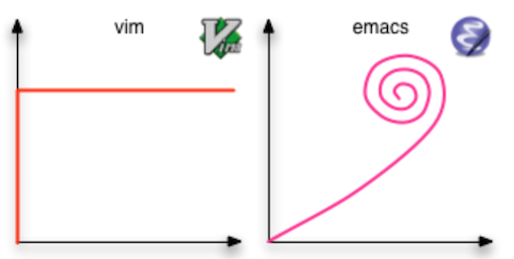
\includegraphics[width=.9\linewidth]{./fig1.png}
\end{center}

这篇笔记简单记录一下spacemacs的安装流程 (Ubuntu 18.04和macOS),基于org-mode的语法和导出为pdf的流程,以及添加spacemacs对中文的支持。最后一点算是重点内容,谷歌了很久找到了相对容易理解的方法。

\section{spacemacs的安装 (Ubuntu和macOS)}
\label{sec:org1bf3e42}
针对spacemacs的安装,参考其github上的\href{https://github.com/syl20bnr/spacemacs\#default-installation}{README}即可,我会简述一下在Ubuntu 18.04 (Linux) 和macOS上的安装和配置方式,目前都是默认配置。

\subsection{Ubuntu 18.04}
\label{sec:org38e2e7a}
针对Ubuntu 18.04的spacemacs安装过程分为以下三步,即

\subsubsection{下载emacs}
\label{sec:org37a984e}
要求版本高于emacs 24,其中Ubuntu14.04貌似不支持,需要独立下载并编译。安装方法如下,
\begin{center}
\begin{verbatim}
$ sudo apt update
$ sudo apt install emacs
# 查看一下版本信息
$ emacs --version
GNU Emacs 25.2.2
Copyright (C) 2017 Free Software Foundation, Inc.
GNU Emacs comes with ABSOLUTELY NO WARRANTY.
You may redistribute copies of GNU Emacs
under the terms of the GNU General Public License.
For more information about these matters, see the file named COPYING.
\end{verbatim}
\end{center}

\subsubsection{配置spacemacs}
\label{sec:org7d7133a}
参考spacemacs的default installation,首先克隆其repository到/home/xxx(这里的xxx是用户名)
\begin{center}
\begin{verbatim}
$ git clone https://github.com/syl20bnr/spacemacs ~/.emacs.d
\end{verbatim}
\end{center}

\subsubsection{安装相关插件}
\label{sec:org650d2f2}
命令行输入emacs初始化spacemacs环境,完成安装。这一步具体安装什么还没太懂,后面慢慢研究一下。\textbf{建议安装过程中选择默认的编辑工具为vim},
个人感觉vim比较适合初学者,掌握几个基本命令就可以工作了。

\subsection{macOS 10.14}
\label{sec:orgac497e6}
针对macOS,我的系统是10.14 Mojave。因为用户习惯,我把macOS的terminal当linux用,所以这里的安装步骤与Ubuntu类似,仅在第一步有区别。
即安装emacs时,采用\texttt{homebrew}工具,具体的命令行写法如下:
\begin{center}
\begin{verbatim}
$ brew install emacs
\end{verbatim}
\end{center}
除此之外,spacemacs官方也提供了安装教程,可以参考\href{https://github.com/syl20bnr/spacemacs\#macos}{这里}。

\section{org-mode的基本语法}
\label{sec:org86742b9}
介绍完spacemacs的安装,便可以开始记笔记了,这里采用的是\href{https://orgmode.org/}{org-mode},org除了提供将文本导出为html和pdf格式外,还可以制作TODO list和日历等,非常适合日常的工作。对于工科孩子,笔记或者小论文的内容主要包含文字、公式、图表、链接和参考文献等,简单举例说明一下他们的语法,详细内容可以参考\href{https://www.cnblogs.com/Open\_Source/archive/2011/07/17/2108747.html}{这篇博客},翻译自org的官方文档,非常详细。我在\href{https://github.com/myinxd/canal-notebooks/blob/master/org-template/org-template.org}{这里}提供了一个与本文内容相同的org笔记以及导出的pdf,感兴趣的话可以作为参考模板。

\textbf{注意:如果要导出pdf,需要预先安装tex套件,建议Texlive},在Ubuntu下可以之间用\texttt{sudo apt install texlive-2016}实现。

\subsection{文档初始化}
\label{sec:org482bb9e}
spacemacs通过文件的后缀名识别文档的类型,对于org-mode,文件的后缀需要为\texttt{.org}。可以采用如下方式初始化笔记并保存,
\begin{center}
\begin{verbatim}
$ emacs notebook.org
\end{verbatim}
\end{center}

\subsection{添加笔记的标题和作者等信息}
\label{sec:org2810a51}
通过在文档头部添加相关的称为"In-buffer settings"的关键字及相关的内容,例如
\begin{verbatim}
#+TITLE: A notebook of spacemacs
#+AUTHOR: Pikachu
#+DATE: 2016-06-11
\end{verbatim}

\subsection{不同级别标题的基本语法}
\label{sec:org561865b}
与markdown类似,org提供了由'*'引导的分级标题的语法规则,例如
\begin{verbatim}
* 一级标题
** 二级标题
*** 三级标题
\end{verbatim}
\subsection{表格}
\label{sec:org8ba9337}
同样的,与markdown类似,org支持添加表格,常用的表格样例如下,
\begin{center}
\begin{verbatim}
| Name  | Phone | Age |
|------ +-------+-----|
| Alice | 12345 | 20  |
| Bob   | 23456 | 21  |
\end{verbatim}
\end{center}

\begin{center}
\begin{tabular}{lrr}
Name & Phone & Age\\
\hline
Alice & 12345 & 20\\
Bob & 23456 & 21\\
\end{tabular}
\end{center}
在表格的填写过程中,有几个快捷键非常好用,例如\texttt{TAB}键用于对齐和增加新的行,其他快捷键建议参考\href{https://www.cnblogs.com/Open\_Source/archive/2011/07/17/2108747.html\#sec-3}{这里}。

\subsection{公式和代码}
\label{sec:org44f9647}
在org-mode下插入公式等价于在latex文档中的操作,直接以equation环境或者\texttt{\$}环境即可,例如
\begin{verbatim}
\begin{equation}
  x = a + b
\end{equation}
\end{verbatim}

\begin{equation}
x = a + b
\end{equation}

插入代码则采用由\texttt{\#+}引导的block,即
\begin{verbatim}
	#+BEGIN_SRC <language>
	code body
	#+END_SRC
\end{verbatim}

显示效果为,
\begin{verbatim}
print("Hello world!")
\end{verbatim}

\subsection{超链接和脚注}
\label{sec:org8d2f9f1}
org对于超链接的支持要优于markdown,能够支持网址、本地文件、文档内部超链接等功能,例如
\begin{verbatim}
# 网址
[[<网址>][<描述>]]
# 本地文件
[[./file.xxx]]
# 文档内部超链接
[[超链接和脚注]]
\end{verbatim}
而脚注的添加方式有两种,即org-mode和基于latex语法的方式,二者在生成的pdf中效果相同。

\begin{verbatim}
# org-mode
引用方式: 这是一个脚注[fn:1],它的位置在本页下方。
脚注格式: [fn:1] 这是一个脚注。

# latex格式
这是一个脚注\footnote{这是一个脚注}
\end{verbatim}

这是基于org-mode的脚注\footnote{这是基于org-mode语法的脚注。}。
这是基于latex语法的脚注\footnote{这是基于latex语法的脚注。}

\subsection{导出为pdf}
\label{sec:org8c4c50c}
最后,需要将记录的文档导出为pdf文件,导出方法是\texttt{Ctrl+c-Ctrl+e-l-p}

\section{添加中文支持}
\label{sec:org6e6ddcd}
受到系统语言设置的限制,spacemacs对于中文的支持存在一些小bug。当系统的语言设定为中文时,直接借助已经安装的拼音输入法便可以实现中文的输入。但是当系统语言为英文时,需要添加对中文的支持。

\subsection{系统语言为英文时如何在spacemacs添加对中文输入法的支持}
\label{sec:org9b5693a}
笔者的系统是Ubuntu18.04,系统语言为英文,安装了fcitx中文中文输入法,在spacemacs中添加中文支持的一种简单方法是在初始化spacemacs时添加如下语句,
\begin{verbatim}
LC_CTYPE=zh_CN.UTF-8 emacs
\end{verbatim}
其中\texttt{LC\_CTYPE}表示本地字符和字符串的编码格式,这里强制设定为中文UTF-8。如果笔记的内容主要为中文,可以在shell的配置文件中固定这一命令,即
\begin{verbatim}
alias emacszh="LC_CTYPE=zh_CN.UTF-8 emacs"
\end{verbatim}

\subsection{解决导出的PDF中文不显示的问题}
\label{sec:org082c310}
在解决spacemacs对中文输入法的支持后,还需要将默认的latex编译命令由\texttt{pdflatex}修改为\texttt{xelatex},因为前者不支持中文。参考emacs-china中的问题,可以通过如下方式修改编译指令,即在文档头部增加,
\#+BEGIN\textsubscript{SRC} emacs
\#END\textsubscript{SRC}
当然,针对这一问题的解决方案还挺多的,多数涉及到LISP的语法和修改spacemacs的配置文件,还是挺麻烦的。

\section{References}
\label{sec:org131ec43}
\begin{enumerate}
\item \href{http://spacemacs.org/\#}{spacemacs}
\item \href{https://github.com/syl20bnr/spacemacs\#default-installation}{spacemacs default installation}
\item \href{https://www.cnblogs.com/Open\_Source/archive/2011/07/17/2108747.html}{Org-mode 简明手册}
\item \href{https://emacs-china.org/t/topic/4465}{Org-mode 添加中文支持}
\item \href{https://emacs-china.org/t/topic/2540}{Orgmode导出PDF显示不了中文}
\end{enumerate}
\end{document}
